\section[M1: Metamodell]{M1: Meta-Modellierung}
\begin{frame}{Meta-Modellierung}
	\centering
	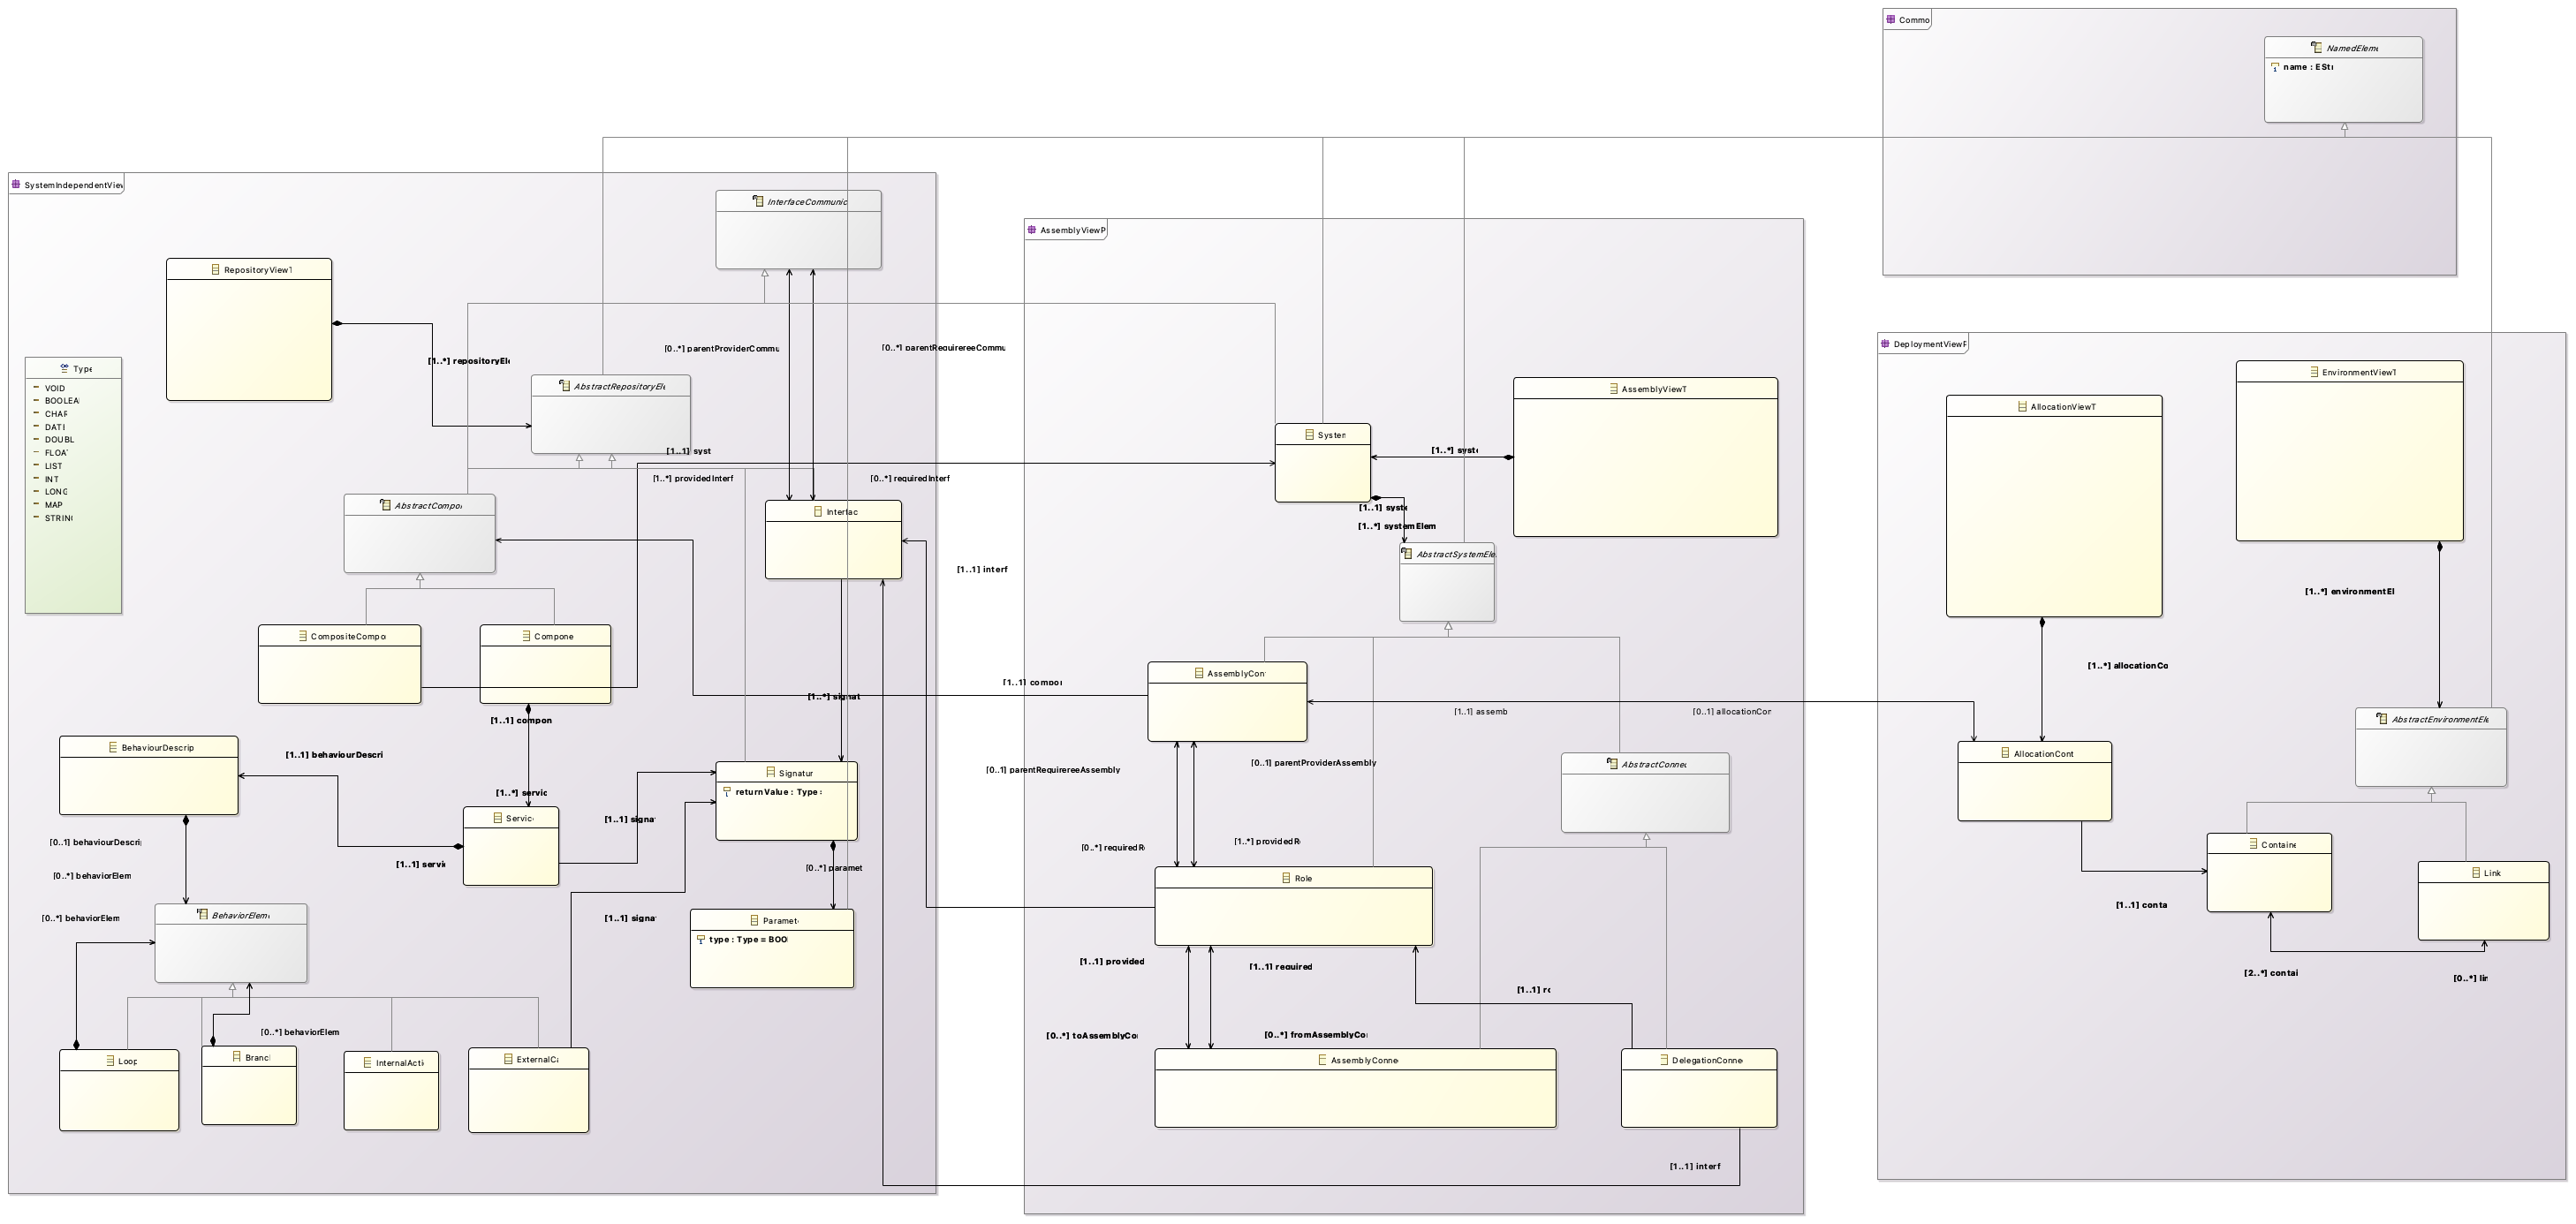
\includegraphics[height=60mm]{figures/meta-modell.png}
\end{frame}

\begin{frame}{Entwurfsentscheidungen für die Meta-Modellierung}
	\begin{itemize}
		\item Verwendung von 4 Packages
		\begin{itemize}
			\item klare Trennung der View Points
			\item Nachteil für spätere Entwicklung
		\end{itemize}
		
		\item Common Package für wiederverwendbare Elemente
		\item ENUM zur Modellierung des \texttt{Type}
		\item Verwendung von OCL
	\end{itemize}
\end{frame}

\begin{frame}{Erstellung der Komponenten für den Media Store}
	\begin{itemize}
		\item mediastore\_allocation.deploymentviewpoint
		\item mediastore\_environment.deploymentviewpoint
		\item mediastore.assemblyviewpoint
		\item mediastore.systemindependentviewpoint
	\end{itemize}
\end{frame}